\input qpd-bootstrap

\begin{problem}{20260728}
  \meta{name}{Cart on a Track}
  \meta{setter}{Elton Liu}
  \meta{score}{15}
  \meta{topic}{mechanics}
  \meta{difficulty}{5}
  \meta{tags}{mechanics, energy, friction, collisions, circular motion, centripetal force, kinematics}

A vertical track smoothly transitions to a horizontal track through a quarter-circle of radius $h$.  A cart is released from rest at height $h$ on the vertical track.  The horizontal track is rough, with kinetic friction coefficient $\mu_k$; the vertical and curved portions are frictionless.

On the horizontal track there is a wall, inclined at an angle $\theta$ to the track's direction (so $\theta$ is the angle between the wall's \emph{surface} and the track, \emph{not} the angle between the wall's normal and the track).  The distance from the start of the horizontal track to the wall is $L_1$.

\begin{center}
  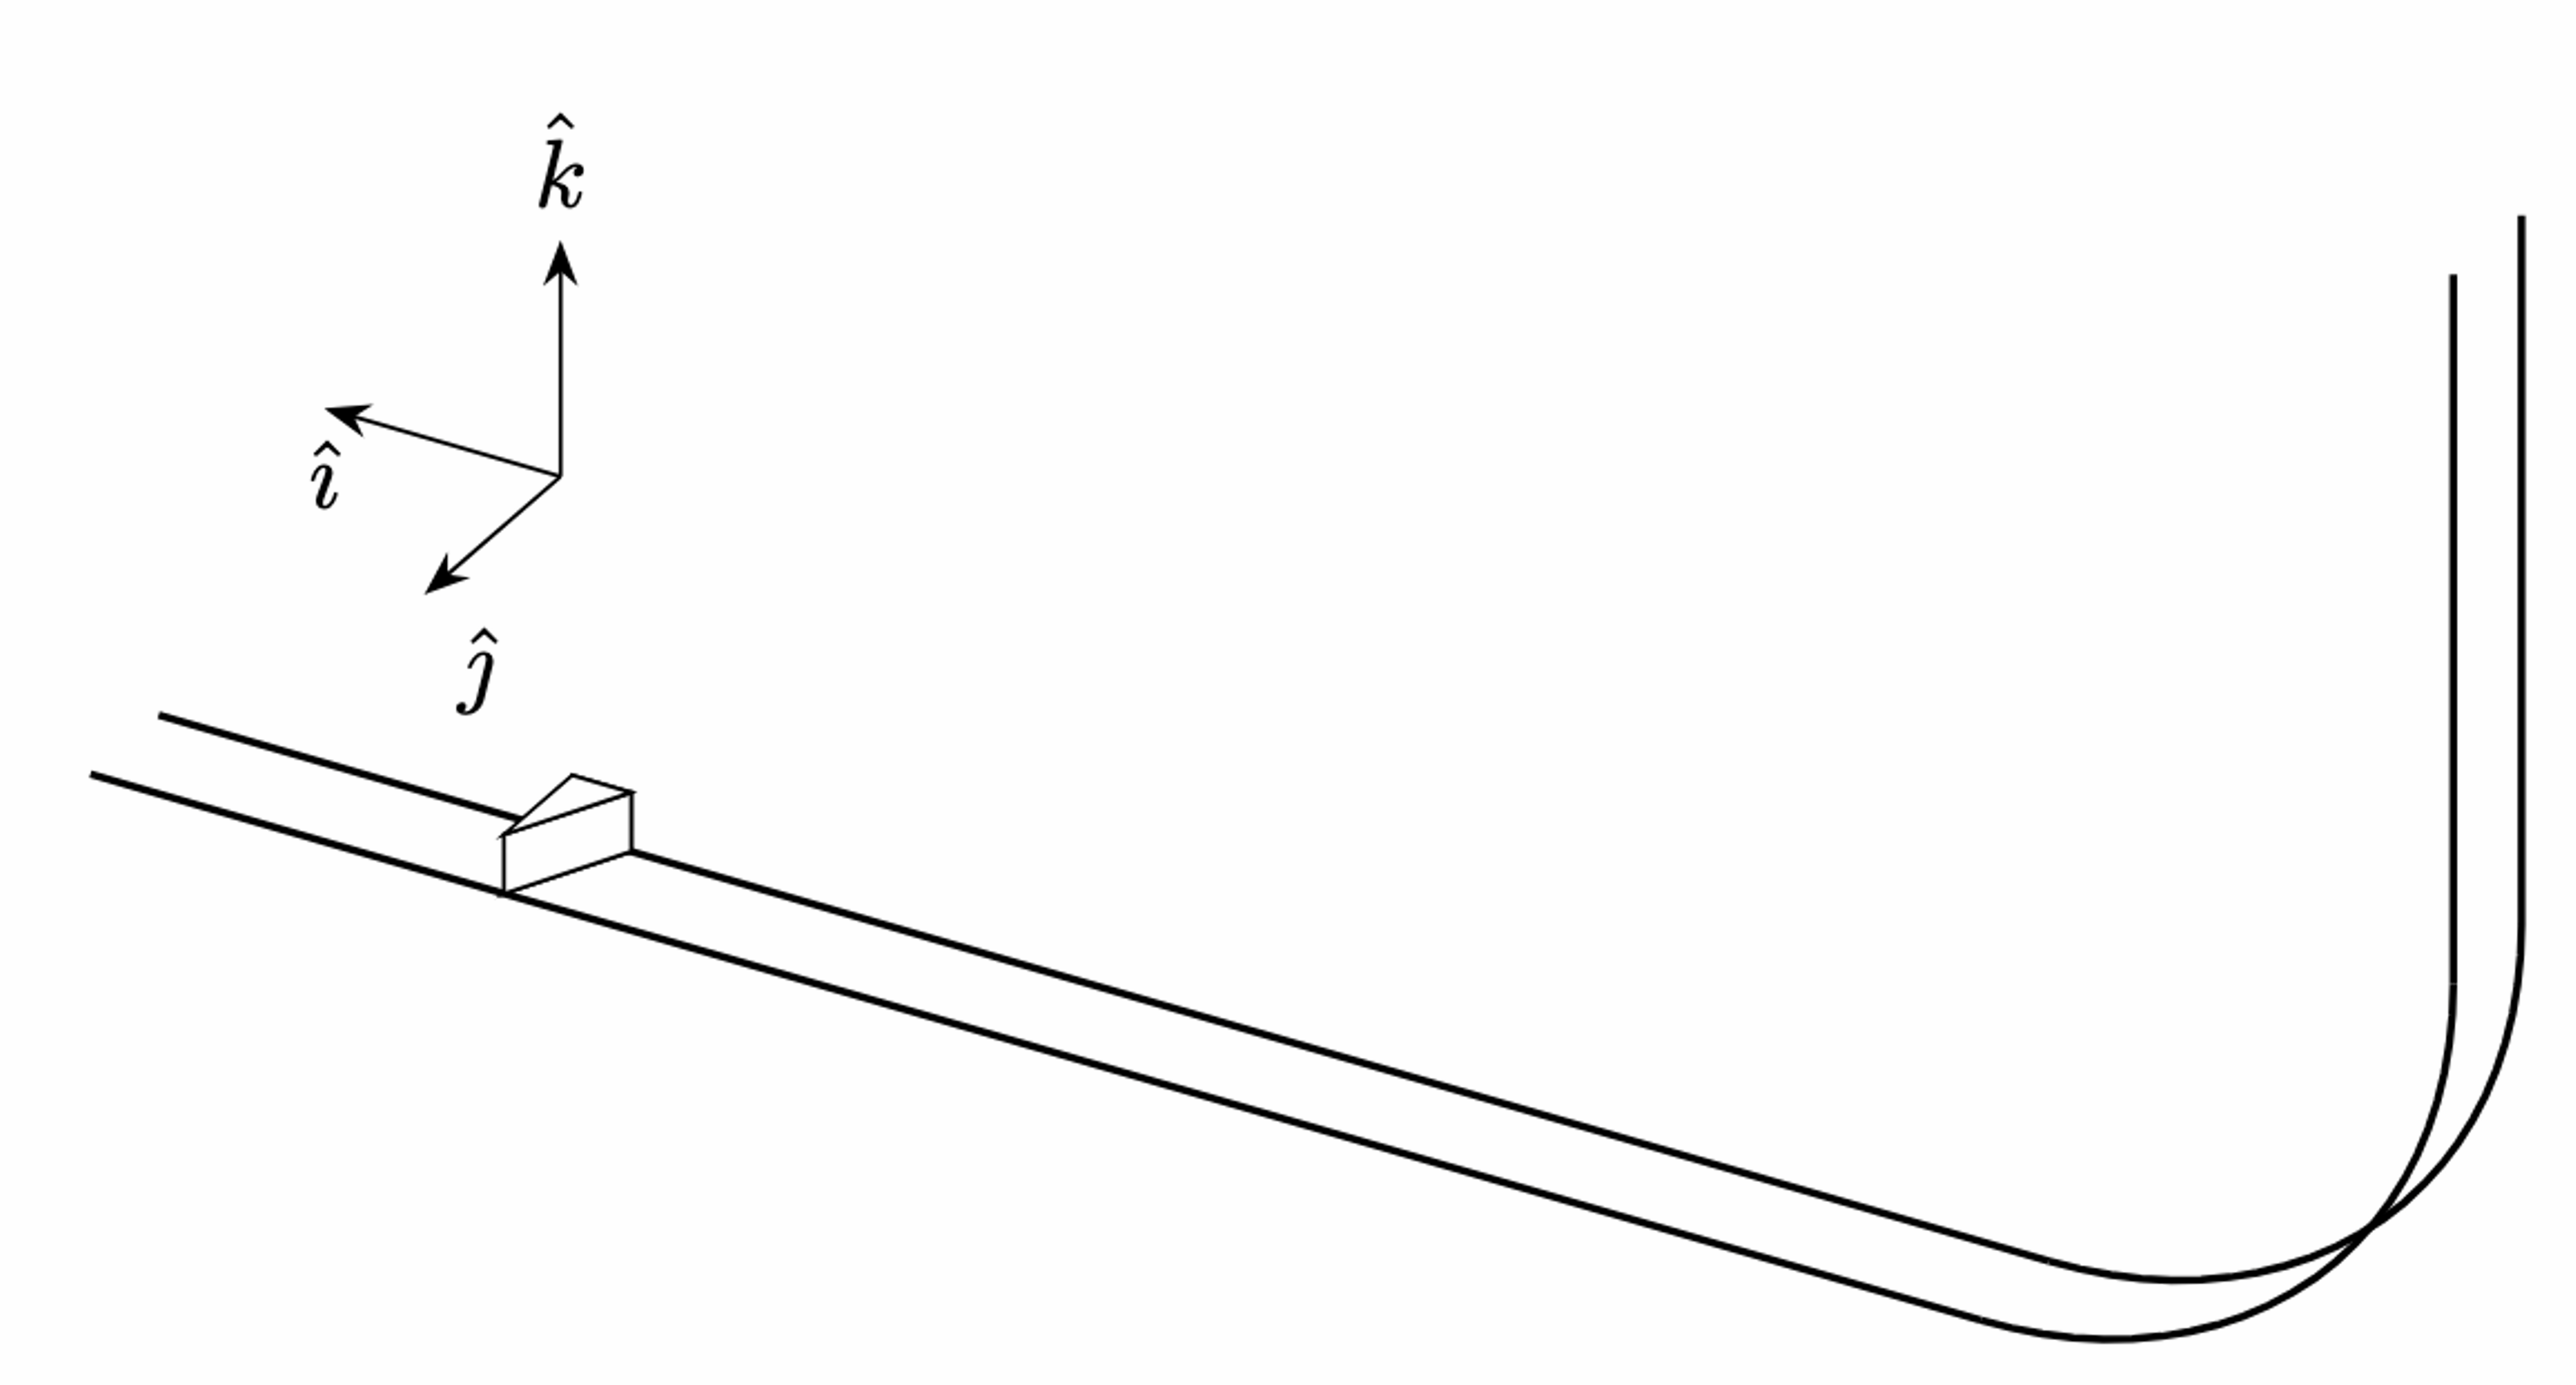
\includegraphics[width=0.6\linewidth]{assets/20260728-1.png}
\end{center}

\begin{assumptions}
  \item The vertical track and the quarter-circle are frictionless; only the horizontal track and the plane after the wall are rough (kinetic friction $\mu_k$).
  \item The wall is smooth and fixed, so the collision is elastic: the velocity component along the wall is unchanged, and the component normal to the wall reverses.  (The cart's speed is therefore unchanged by the collision.)
  \item The cart is a point mass; it never leaves the track during the descent.
\end{assumptions}

\begin{questions}
  \item \textbf{Entry speed.}
        Using conservation of energy, find the speed $v_0$ of the cart just as it begins moving on the horizontal track.

  \item \textbf{Speed before the wall.}
        Find the speed $v_1$ of the cart just before it reaches the wall.

  \item \textbf{After the collision.}
        Find the $x$- and $y$-components of the velocity vector after the collision, taking $+x$ along the track and $+y$ perpendicular to it in the horizontal plane.

  \item \textbf{Sliding to rest.}
        After the collision the cart slides on the flat plane (the same material as the horizontal track).  Find the distance it covers after the collision before stopping.

  \item \textbf{Maximum acceleration.}
        Find the maximum acceleration the cart experiences after it begins to move on the track.

  \item \textbf{Total path length.}
        Find the total distance (path length) covered by the cart after release.

  \item \textbf{Total displacement.}
        Find the total displacement of the cart after release (i.e. the vector from the release point to the final stopping point).
\end{questions}

\end{problem}

\begin{solution}{20260728}

\subsection*{Q1. Entry speed}

The descent is frictionless and the total drop is $h$, so by conservation of energy
\[
  mgh = \tfrac12 m v_0^{2}
  \;\Longrightarrow\;
  \boxed{v_0 = \sqrt{2gh}}.
\]

\subsection*{Q2. Speed before the wall}

On the rough horizontal track the kinetic friction is $\mu_k m g$, giving a deceleration $\mu_k g$ over distance $L_1$:
\[
  v_1^{2} = v_0^{2} - 2\mu_k g L_1 = 2g(h - \mu_k L_1)
  \;\Longrightarrow\;
  \boxed{v_1 = \sqrt{2g\bigl(h - \mu_k L_1\bigr)}}.
\]

\subsection*{Q3. After the collision}

The incoming velocity is $(v_1, 0)$ along $+x$.  For a smooth wall whose surface makes angle $\theta$ with $+x$, the tangential component $v_1\cos\theta$ is preserved and the normal component $-v_1\sin\theta$ reverses.  Recombining,
\[
  \mathbf{v}' = v_1\cos\theta\,\hat{\mathbf{t}} + v_1\sin\theta\,\hat{\mathbf{n}}
              = v_1\bigl(\cos 2\theta,\ \sin 2\theta\bigr),
\]
so
\[
  \boxed{v_x = v_1\cos 2\theta, \qquad v_y = v_1\sin 2\theta},
\]
with $v_1$ from Q2.  (For $\theta = 90^{\circ}$ the cart bounces straight back; for $\theta = 45^{\circ}$ it leaves at $90^{\circ}$ to the track.)

\subsection*{Q4. Sliding to rest}

The collision is elastic, so the speed is still $v_1$; the cart now slides on the plane with friction $\mu_k g$.  The stopping distance is
\[
  d = \frac{v_1^{2}}{2\mu_k g}
    = \frac{2g(h - \mu_k L_1)}{2\mu_k g}
    = \boxed{\frac{h}{\mu_k} - L_1}.
\]

\subsection*{Q5. Maximum acceleration}

On the frictionless quarter-circle the acceleration has magnitude
\[
  a = \sqrt{a_t^{2} + a_c^{2}},
  \qquad
  a_c = \frac{v^{2}}{h}, \quad a_t = g\cos\varphi ,
\]
where $\varphi$ is measured from the top of the circle.  Using $v^{2} = 2gh(1-\cos\varphi)$,
\[
  \frac{a^{2}}{g^{2}} = \cos^{2}\varphi + 4(1-\cos\varphi)^{2},
\]
which is maximised at $\varphi = \pi/2$ (the bottom), where $a_c = v_0^{2}/h = 2g$ and $a_t = 0$.  The vertical track gives only $g$ and the horizontal track only $\mu_k g < g$, so
\[
  \boxed{a_{\max} = 2g}.
\]

\subsection*{Q6. Total path length}

The path consists of the quarter-circle arc, the straight run to the wall, and the post-collision slide:
\[
  L_{\text{tot}} = \frac{\pi}{2}h + L_1 + d
  = \boxed{\frac{\pi}{2}h + \frac{h}{\mu_k}},
\]
using $d = h/\mu_k - L_1$ (the $L_1$ terms cancel).

\subsection*{Q7. Total displacement}

Take $+x$ along the track toward the wall, $+y$ horizontal perpendicular to the track, and $+z$ vertically upward.  The release point is at $(-h, 0, h)$ (the top of the quarter-circle), and the final stopping point is at
\[
  \bigl(L_1 + d\cos 2\theta,\ d\sin 2\theta,\ 0\bigr).
\]
Therefore the displacement vector is
\[
  \boxed{\Delta\mathbf{r}
  = \Bigl(L_1 + d\cos 2\theta + h,\ d\sin 2\theta,\ -h\Bigr)},
\]
with $d = h/\mu_k - L_1$, and its magnitude is
\[
  \boxed{\lvert\Delta\mathbf{r}\rvert
  = \sqrt{\bigl(L_1 + d\cos 2\theta + h\bigr)^{2} + \bigl(d\sin 2\theta\bigr)^{2} + h^{2}}}.
\]

\end{solution}

\input qpd-end
